% !TEX root = domain_transduction.tex
We address the problem of unsupervised transductive domain adaptation by jointly solving for the label assignment of unsupervised target domain as well as the shift between the domains. We first define our model in Section~\ref{prob:def} and explain the two sub-problems of transduction and adaptation. We further explain the details of transduction in Section~\ref{label} and the details of adaptation in Section~\ref{metric}.
%Unsupervised domain adaptation is inherently a transduction problem since the main challenge lies in labeling the unsupervised data points with the help of the supervised data; because, adaptation is done offline without computationally concerns and the accuracy is critical since the transduction error is a good proxy for generalization \cite{adapttheory}. Main complication, which makes existing transduction methods inapplicable, is the domain shift between the supervised and unsupervised data points . We explicitly model the domain shift and jointly solve for unsupervised labels as well as the domain shift in a transductive learning setup.

\subsection{Problem Definition and Notation}
\label{prob:def}
In the unsupervised domain adaptation problem, one of the domains (source) is fully supervised $\{\xsi, \ysi \}_{i \in [N^s]}$ with $N^s$ data points $\xsi$ and corresponding labels $\ysi$ from a discrete set $\ysi \in \{1,\ldots, Y \}$.  The other domain (target), on the other hand is unsupervised and has $N^u$ data points $\{\xui \}_{i \in [N^u]}$. 

We further assume that both domains have different distributions $\xsi \sim p_s$ and $\xui \sim p_t$ defined on the same space as $\xsi,\xui \in \mathcal{X}$. We consider a case in which there are two feature functions  \mbox{$\Phi_s, \Phi_t:\mathcal{X}\rightarrow \mathcal{R}^d$} applicable to source and target separately. These feature functions extracts both the information shared among domains and explicit to the individual ones. The way we model common features is sharing a subset of parameters between feature functions as \mbox{$\Phi_s=\Phi_{\theta_c,\theta_s}$} and \mbox{$\Phi_t=\Phi_{\theta_c,\theta_t}$}. We use deep neural networks to implement these functions and in our implementation $\theta_c$ corresponds to the parameters in the first few layers of the networks and $\theta_s$, $\theta_t$ corresponds to the respective final layers. In general, our model to applicable any hierarchical and differentiable feature function which can be expressed as a composite function $\Phi_s = f_{\theta_s}(g_{\theta_c}(\cdot))$ for source and similarly for target.

\subsection{Consistent Structured Transduction}
% talk about cyclic consistency and structured consistency
Our model is based on modeling the domain shift in terms of a metric function and further jointly solving for labels of the unsupervised data-points and the metric function. As a similarity metrics, we use the inner product as $s(\xsi, \xuj) = \Phi_s(\xsi)^\intercal \Phi(\xuj)$. We denote the two main components of our method as transduction and adaptation. The transduction is the sub-problem of labelling unsupervised data points and the adaptation is solving for the domain shift. In order to solve this joint problem tractably, we exploit two heuristics; cyclic consistency for transduction and structured consistency for adaptation. 

\textbf{Cyclic consistency:} One desired property of  $\Phi_s$ and $\Phi_t$ is their consistency. If we estimate the labels of the unsupervised data points and further use these points to estimate the labels of supervised data-points, we want the predicted labels of the supervised data-points to be consistent with the ground truth labels. In other words;

\begin{displaymath}
    \xymatrix{
        (\xsi,\ysi) \ar@{<->}@<-2pt>`d[r] `[rrrrrr]|{\textbf{Cyclic Consistency: $\ysi = \ysi^{pred}$}} [rrrrrr]  \ar[rrr]|{\textbf{Transduction}}     &&& (\xui, \yui^{pred}) \ar[rrr]|{\textbf{Transduction}} &&&  (\xsi,\ysi^{pred}) }
\end{displaymath}

We can formally represent the cyclic consistency in terms of a large-margin nearest neighbor (LMNN)\cite{lmnn} rule if transduction follows a nearest neighbor rule. For each source point, we enforce a margin between its similarity with the nearest neighbor from the target having the same label and having a different label as; $ \Phi_s(\xsi)^\intercal \Phi_t(\mathbf{x}_{i^+}) > \Phi_s(\xsi)^\intercal \Phi_t(\mathbf{x}_{i^-}) + \alpha$ where $\mathbf{x}_{i^+}$ is the nearest target having the same class as $\xsi$ and $\mathbf{x}_{i^-}$ is the nearest target having a different class label. 


\textbf{Structured consistency:} We enforce a consistency in labelling of the target data-points during the transduction. In other words, if two target data-points are similar to each other, they are more likely to have same label. In order to enforce this consistency, we create a k-NN graph of target data points using a similarity metric $\Phi_t(\xui)^\intercal \Phi_t(\xuj)$. We denote the neighbors of the point $\xsi$ as $\mathcal{N}(\xsi)$. We enforce structured consistency by penalizing neighbor points of same labels with their similarity score. 

Our model leads to the following optimization problem, over the target labels $\yui$ and the feature function parameters $\theta_c, \theta_s, \theta_t$, jointly solving transduction and adaptation. 
\begin{equation}
\small
\begin{aligned}
\min_{\substack{\theta_c,\theta_s,\theta_t, \\ y_1, \ldots y_{N^u}}} &\sum_{i \in [N^s]} [\Phi_s(\xsi)^\intercal \Phi_t(\mathbf{x}_{i^-}) -\Phi_s(\xsi)^\intercal \Phi_t(\mathbf{x}_{i^+}) + \alpha]_{+}  +\lambda \sum_{i \in [N^u]} \sum_{\xuj \in \mathcal{N}(\xui)}  \Phi_t(\xui)^\intercal \Phi_t(\xuj) \mathds{1}(y_i \neq y_j)\\
% \Phi(\xui)^\intercal \Phi(\xuj) \mathds{1}(y_i \neq y_j)\\
s.t. &\quad i^{+} = {\arg\max}_{j | y_j = \hat{y}_i} \sw(\mathbf{\hat{x}}_i,\mathbf{x}_{j}) \\
&\quad i^{-} = {\arg\max}_{j | y_j \neq \hat{y}_i} \sw(\mathbf{\hat{x}}_i,\mathbf{x}_{j}) 
\end{aligned}
\label{loss}
\end{equation}
where $\mathds{1}(a)$ is an indicator function which is $1$ if $a$ is true and $0$ otherwise. $[a]_+$ is a rectifier function which is equal to $\max(0, a)$.

We solve this optimization problem via alternating minimization through iterating over solving for unsupervised labels $y_i$(transduction) and learning the similarity metric $\theta_c,\theta_s,\theta_t$ (adaptation). We explain these two steps in detail in the following sections.


\iffalse
\begin{wrapfigure}{r}{0.5\textwidth}
    \begin{minipage}{0.5\textwidth}
    \vspace{-1cm}
\begin{algorithm}[H]
   \caption{Transduction with Domain Shift}
   \label{alg:example}
\begin{algorithmic}
   \STATE {\bfseries Input:} source $\mathbf{x}_i$, target $\mathbf{\hat{x}}_i$, $y_i$, batch size $B$
   \REPEAT
   \STATE  Sample $\{\mathbf{x^b}_{1 \cdots B}\}$, $\{\mathbf{\hat{x}}^b_{1 \cdots B}, \hat{y}^b_{1\cdots B}\}$
   \STATE Solve (\ref{robtran}) for $\{y_{1 \cdots B}\}$
   \FOR{$i=1$ {\bfseries to} $B$}
      \IF{$ \hat{y}_i \textbf{ in } y_{1 \cdots y_B} $} 
   \STATE Compute ($i^+, i^-$) using $\{y_{1 \cdots B}\}$ in (\ref{sup_nn})
   \STATE Update $\frac{\partial loss}{\partial \mathbf{\theta}}$ and  $\frac{\partial loss}{\partial \mathbf{W}} $ using (\ref{gradw},\ref{gradt})
   \ENDIF
   \ENDFOR
   \STATE $\mathbf{W} \leftarrow \mathbf{W} + \alpha \frac{\partial loss (y_i, \mathbf{W})}{\partial \mathbf{W}}$ 
   \STATE $\mathbf{\theta} \leftarrow \mathbf{\theta} + \alpha \frac{\partial loss (y_i, \mathbf{W})}{\partial \mathbf{\theta}}$
   \UNTIL CONVERGENCE or $MAX\_ITER$
\end{algorithmic}
\end{algorithm}
\vspace{-1cm}
  \end{minipage}
  \end{wrapfigure}
\fi





 %} $ 

%$\max_{y_1} \$
%$\min_{y_1} + 
%_4) $ assuming green is $0$, blue is $1$ and red is $2$

\subsection{Transduction: Labeling Target Domain}
\label{label}
In order to label the unsupervised points, we use the k-nearest-neighbor rule. We simply compute the k-NN supervised data point for each unsupervised data point using the learned metric and transfer the corresponding majority label. Formally, given a similarity metric $\theta_c, \theta_s, \theta_t$, the k-NN rule is 
$(y_i)^{pred} = \arg\max_y \frac{k_y(\xui)}{k}$ where $k_y(\xui)$ is the number of samples having label $y$ in the $k$ nearest neighbor of $\xui$ from the source set. 

One major issue with this approach is the accuracy of transduction during the initial stage of the algorithm. Since the learned metric will not be accurate, we expect to see some noisy k-NN sets. Hence, we propose two solutions to solve this problem.

\textbf{Structured Consistency:} We use label propagation to enforce consistency of the predicted labels of unsupervised data points. Similar to existing graph transduction algorithms \cite{label_prop1,label_prop2}, we create a k-nearest neighbor (k-NN) graph over the unsupervised data points and penalize disagreements of labels between neighbors.

\textbf{Reject option:} In the initial stage of the algorithm, we let transduction step to use reject $R$ as a label to unsupervised target points. In other words, our transduction algorithm can decide to not label some of the points so that they will not be used for adaptation. When the learned metric gets more accurate in the future iterations, transduction algorithm can label these rejected points.

We define our transduction sub-problem as:

\begin{equation}
\begin{aligned}
\min_{y_1, \ldots y_{N^u} \in [Y] \cap R}  &\sum_{i \in N^u} l(\xui, y_i) + \lambda \sum_{i \in N^u} \sum_{\xuj \in \mathcal{N}(\xui)} \Phi_s(\xui)^\intercal \Phi_t(\xuj)\mathds{1}(y_i \neq y_j)
\end{aligned}
\label{robtran}
\end{equation}

where $l(\xui, y) = \left\{ \begin{array}{cc}  1 - \frac{k_y(\xui)}{k} & y \in [Y] \\ \gamma \max_{y^\prime \in [Y]} \frac{k_y^\prime(\xui)}{k}
 & y=R \end{array}\right.$ and $\gamma \geq 1$ is relative cost of reject option. 
 
The $l(\xui,R)$ is smaller if none of the class has a majority, promoting reject option for undecided cases. We also modulate the $\gamma$ during learning to decrease number of reject options in the later stage of the adaptation. This problem can approximately be solved using many existing methods. We use the $\alpha$-$\beta$ swapping algorithm from \cite{kolmogrovalphabeta} since it is experimentally shown to be efficient and accurate. In order to further explain the label propagation, we visualize an example with $k=4$ and $4$-class classification problem in Figure~\ref{vis_label_prop}. 

\begin{wrapfigure}{r}{0.5\textwidth}
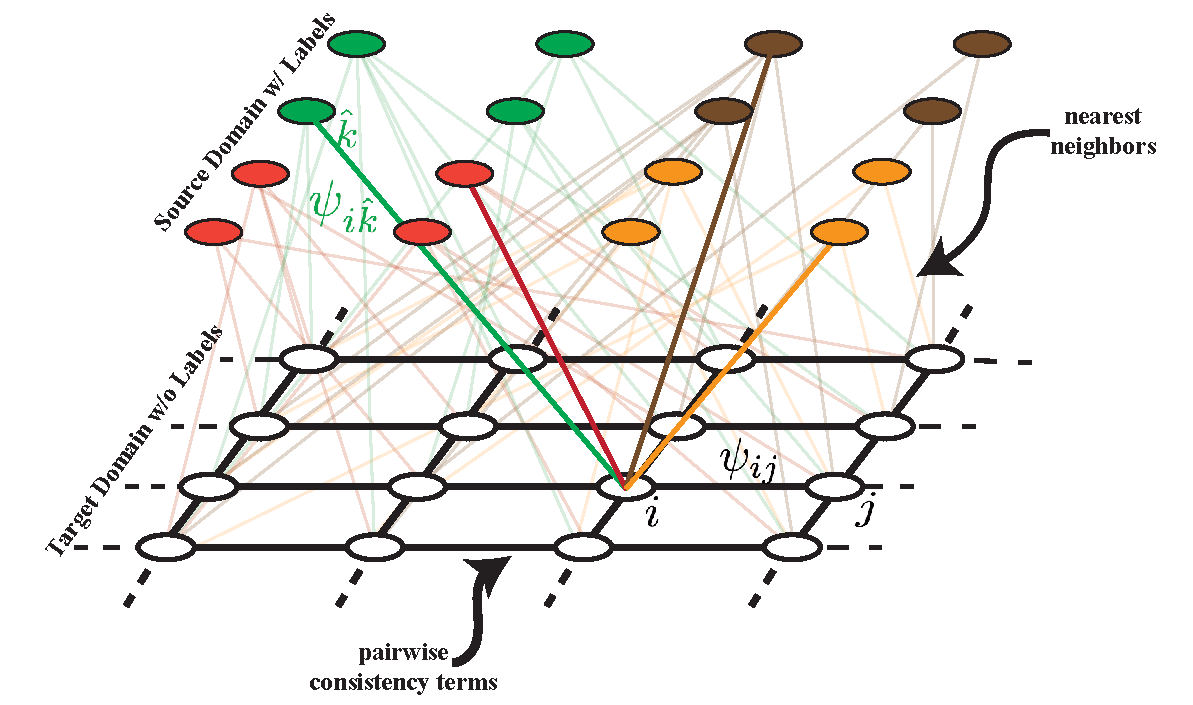
\includegraphics[width=0.5\textwidth]{fig11}
\caption{\textbf{Visualization of the Label Propogation.} We create a k-NN graph of unsupervised target points to enforce consistency with pairwise terms 
\mbox{$\psi_{ij}=sim(\mathbf{x}_i, \mathbf{x}_j) \mathds{1}(y_i \neq y_j)$} and use closest supervised source points to each class as 
\mbox{$ \psi_{i\hat{k}} \sw(\mathbf{\hat{x}}_k,\mathbf{x}_{i})$}.} 
\vspace{-1cm}
\label{vis_label_prop}
\end{wrapfigure}


It is also critical that this formulation requires solving high number of nearest neighbors which is computationally challenging. Fortunately, we use stochastic gradient descent in our adaptation stage with a carefully chosen batch size, which requires us to only solve the transduction over a batch. %Furthermore, we also efficiently implement the distance computation in the form of a few OpenBLAS calls as we further explain in detail in Section~\ref{imp_det}.

\subsection{Adaptation: Learning the Metric}
\label{metric}
Given the predicted labels $y_i$ for unsupervised data points $\xui$, we need to learn an asymmetric metric in order to minimize the loss function defined in (\ref{loss}). 

The main intuition behind our formulation is to seek a metric which can label the supervised points correctly using the unsupervised points and their predicted labels. In other words, we reverse the labeling direction. At this stage we have already predicted a label for each unsupervised point; hence, we can estimate a label for each supervised point using the predicted labels. We also have ground truth labels for the supervised points and we combine them to find an asymmetric metric. In other words, the goal of the adaptation stage is:

\vspace{-3mm}
\begin{itemize}
\item predicting $\hat{y}^{pred}_j$ using $\xui, \xsj, \yui$
\item learning $\sw(\cdot,\cdot)$ by penalizing  $(\hat{y}_j)^{pred} \neq \hat{y}_j$ 
\end{itemize}

Fortunately, this can be jointly solved by minimizing the triplet loss defined with supervised data points and their closest same class and different class neighbors among the unsupervised points. Formally, we find the closest same class and different class points as;
\begin{equation}
\begin{aligned}
&i^{+} = {\arg\max}_{j | y_j = \hat{y}_i} \sw(\xsi, \xui) \\
&i^{-} = {\arg\max}_{j | y_j \neq \hat{y}_i} \sw(\xsi,\xuj) 
\label{sup_nn}
\end{aligned}
\end{equation}

  
We further define the loss function with a regularizer using the nearest neighbors as: $loss(\mathbf{W})=$
\begin{equation}
%\min_{\mathbf{W}}
 \sum_{i \in [N^s]} [\sw(\mathbf{\hat{x}}_i,\mathbf{x}_{i^-}) - \sw(\mathbf{\hat{x}}_i,\mathbf{x}_{i^+}) + \alpha]_{+} + r(\mathbf{W})
\end{equation}
which is convex in terms of the $\mathbf{W}$ if the regularizer is convex; and we optimize it via stochastic gradient descent using the subgradient \
\mbox{$\frac{\partial loss (y_i, \mathbf{W})}{\partial \mathbf{W}} = \frac{\partial r ( \mathbf{W})}{\partial \mathbf{W}} + $}
%\begin{small}
\begin{equation}
\begin{aligned}
\sum_{i \in [N^s]} &\mathds{1}(\sw(\xsi,\mathbf{x}_{i^-}) - \sw(\xsi,\mathbf{x}_{i^+})>\alpha) \\
&\times \left( \Phi(\xsi)\Phi(\mathbf{x}_{i^-})^\intercal - \Phi(\xsi)\Phi(\mathbf{x}_{i^+})^\intercal  \right)  
\end{aligned}
\label{gradw}
\end{equation}
%\end{small}
%\end{small}
As a regularizer use the Frobenius norm of the similarity matrix as $r(\mathbf{W})=\frac{1}{2}\|\mathbf{W}\|_F^2$. We explain the details of this optimization routine in the Section~\ref{imp_det}.


\subsection{Learning Features}
In Section~\ref{label}~and~\ref{metric}, we explained our transduction with label propagation as well as the adaptation algorithm using a pre-defined feature function $\Phi$. However, the current trends in machine learning suggest that learning this feature function $\Phi$ from the data using deep neural networks is a promising direction especially for visual domains. Hence, we consider the case where $\Phi_{\mathbf{\theta}}$ is a parametrized feature function with parameter set, $\mathbf{\theta}$. A typical example is CNNs (Convolutional Neural Networks) with $\mathbf{\theta}$ as concatenation of weights and biases in the layers of CNN. We learn the feature function parameters as part of the adaptation stage with an update; $\frac{\partial loss (y_i, \mathbf{W})}{\partial \mathbf{\theta}} =$

\begin{small}
\begin{equation}
\begin{aligned}
 \sum_{i \in [N^s]} &\mathds{1}(\sw(\xsi,\mathbf{x}_{i^-}) - \sw(\xsi,\mathbf{x}_{i^+})>\alpha)  \\
 &\times \left(\frac{\partial \sw(\xsi,\mathbf{x}_{i^-}) }{\partial \mathbf{\theta}} - \frac{\partial \sw(\xsi,\mathbf{x}_{i^+}) }{\partial \mathbf{\theta}} \right)
 \label{gradt}
 \end{aligned}
\end{equation}
\end{small}
where {\small $\frac{\partial \sw(\xsi,\xuj) }{\partial \mathbf{\theta}} =\Phi(\xuj)^\intercal \mathbf{W}^\intercal \frac{\partial \phi_\mathbf{\theta}(\xsi)}{\partial \theta} + \Phi(\xsi)^\intercal \mathbf{W} \frac{\partial \phi_\mathbf{\theta}(\xuj)}{\partial \theta} $}

  